\documentclass[conference]{IEEEtran}

\usepackage{amsmath}
\usepackage{graphicx}
%\usepackage[backend=bibtex,style=chem-rsc]{biblatex}
\usepackage{lettrine}
\usepackage{cite}
\usepackage{float}
\usepackage{blindtext}
\usepackage{eso-pic}
\usepackage[utf8]{inputenc}
\usepackage[english]{babel}
\usepackage[numbers]{natbib}
\usepackage{hyperref}
\usepackage{booktabs}
\usepackage{filecontents}
\newcommand\tab[1][1cm]{\hspace*{#1}}
\newcommand\AtPageUpperMyright[1]{\AtPageUpperLeft{%
    \put(\LenToUnit{0.5\paperwidth},\LenToUnit{-1cm}){%
     \parbox{0.5\textwidth}{\raggedleft\fontsize{9}{11}\selectfont #1}}%
    }}%
    \newcommand{\conf}[1]{%
    \AddToShipoutPictureBG*{%
    \AtPageUpperMyright{#1}}
}

\title{Sample paper}

\author{
  \IEEEauthorblockN{Armaan Kohli}
  \IEEEauthorblockA{\textit{Department of Electrical Engineering} \\
\textit{The Cooper Union for the Advancement of Science and Art}\\
New York City, United States \\
kohli@cooper.edu\\
\href{github.com/armaank/wi-comms}{https://github.com/armaank/wi-comms}}}

\begin{document}
\title{MIMI-OFDM Wireless Link Simulations}

\maketitle
\conf{ECE-408: WIRELESS COMMUNICATIONS, April 2020}

\begin{abstract}
 We simulate a MIMO wireless link and implement a simple OFDM scheme based on the IEEE802.11a standard with several different types of equalization techniques. We then design a MIMO-OFDM system and conduct a performance analysis of the wireless link. 
\end{abstract}

\begin{IEEEkeywords}
MIMO, OFDM, MIMO-OFDM, IEEE802.11a, channel estimation, zero-forcing equalization, minimum mean-squared error equalization.

\end{IEEEkeywords}

\section{Introduction}
\lettrine[findent=2pt]{\textbf{M}}{ }IMO-OFDM is a technique used in large scale wireless systems. MIMO, multi-input mutli-output, in the context of communications, means that the system consists of multiple transmitters and multiple receivers. OFDM, orthogonal frequency division multiplexing, is a technique used to increase throughput by transmitting data across multiple frequencies. 

\section{MIMO Link}
MIMO wireless channels differ from SISO channels in that the MIMO channel must be represented as a matrix $H$, called the channel matrix. Thus, we can write the output of the MIMO channel as: 
\begin{equation}
y = Hx + v
\end{equation}
Where $v$ is an additive white Gaussian noise (awgn) vector. This is the representation of a wireless MIMO link. 
\subsection{Channel Precoding}
The first method for channel equalization is called precoding. Pre-coding uses the matrix representation of the channel to code the transmitted and received signal in such a way that we orthogonalize the channel. 
Let $N$ denote the number of channel
If $H$ is full rank, then we can compute the singular-value decomposition (SVD) of the channel matrix as 
\begin{equation}
H = U\Sigma V^H
\end{equation}
By pre-multiplying our signal by $V$, and then post-multiplying our signal by $\Sigma^{-1} U^H$, we can orthogonalize our channel, so that each different signal is placed on independent channels, reducing interference.
 However, this method requires perfect channel state information at the transmitter (CSIT), which isn't feasible in realizable systems. In practice, a least squares approach could be used instead. 

\subsection{ZF Equalization}
Instead of performing channel precoding, one could increase the performance of a MIMO system via zero-forcing (ZF) equalization. This has the advantage that it doesn't require CSIT, only channel state information at the receiver (CSIR), which is more realistic in practice. ZF equalization using the least squares (LS) solution to compute a filter to apply at the reciever to correct for interference effects. 
\begin{equation}
W_{ZF} = (H^HH)^{-1}H^H 
\end{equation}
This is a good choice because it is a minimum variance unbiased estimator, and doesn't make any assumptions about the distribution of $v$, the noise in the channel.
\subsection{MMSE Equalization}
Minimum mean-squared-error, on the other hand, makes use of an a-priori assumption that $v$ is Gaussian distributed in order to construct a filter to apply at the receiver to minimize the error. Again, this solution assumes CSIR.
\begin{equation}
W_{MMSE} = (H^HH + \sigma_n I)^{-1}H^H 
\end{equation}
\subsection{Results}
We simulated a 2x2 MIMO link over three random Gaussian flat fading channel, using each of the aforementioned equalization techniques. Fig. \ref{fig:mimo} shows waterfall curves evaluating the bit error rate of the scheme for a set of EbNo values. The link used a 16-QAM modulation scheme.
\begin{figure}[htbp]
\centerline{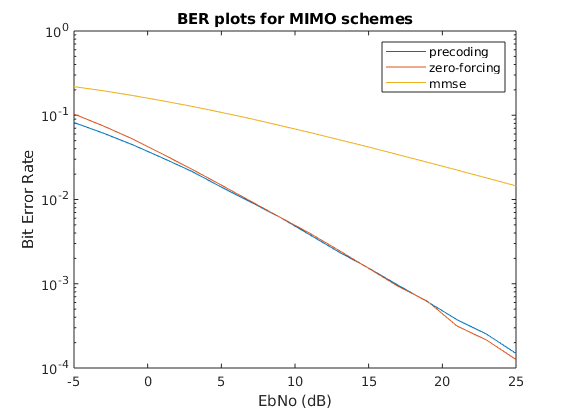
\includegraphics[scale=.4]{./media/mimo_01.png}}
\caption{Comparing BER of different equalization schemes for a 2x2 MIMO link}
\label{fig:mimo}
\end{figure}\\
As expected, pre-coding achieved the best performance, while ZF equalization allows comparable performance while not making such strong assumptions.
\section{OFDM}
OFDM uses orthogonal frequencies to increase the throughput of a wireless link. This method also leverages matrix representation, making MIMO and OFDM a natural couple. 

An OFDM burst is constructed by taking an N-point IFFT of the the input data message, which places the data on N orthogonal frequency bands. Thus, we can represent the output of an OFDM system is 
\begin{equation}
y = Hx + v
\end{equation}
Where H is a normal matrix, and the dimension of H corresponds to the number of points in the IFFT. This is identical to the formulation of MIMO. We modelled our OFDM system on the 802.11a standard.

\subsection{802.11a PHY Layer Overview}
A single OFDM burst according to 802.11a consists of 80 total symbols. 16 symbols are dedicated to the cyclic prefix, leaving the remaining 64 symbols for data. Of the 64 symbols, 12 of them coorespond to the gaurd interval, 4 are dedicated for carrier symbols and 48 symbols for actual data \cite{goldsmith}. The actual indices in the OFDM burst for the data and pilot sequences is specified in the 802.11a standard. 

\subsection{ZF Equalization}
ZF equalization for a OFDM system consists of a dividing the received OFDM frame by the channel coefficients. This is because the OFDM operates in the frequency domain. This method assumes CSIR, and doesn't encode any prior on the noise distribution.
\begin{equation}
W_{zf}[i] = \frac{1}{H[i]}
\end{equation}

\subsubsection{MMSE Equalization}
MMSE for an OFDM system normalizes the response to unit magnitude, and assumes the noise is Gaussian distributed. 
\begin{equation}
W_{mmse}[i] = \frac{H[i]^*}{H[i]H[i]^* + v[i]}
\end{equation}
\subsubsection{Results}
We simulated an OFDM system over three Rayleigh fading channels, using ZF and MMSE equalization. Fig. \ref{fig:ofdm} shows waterfall curves evaluating the bit error rate of the scheme for a set of EbNo values. The link used a 16-QAM modulation scheme.
\begin{figure}[htbp]
\centerline{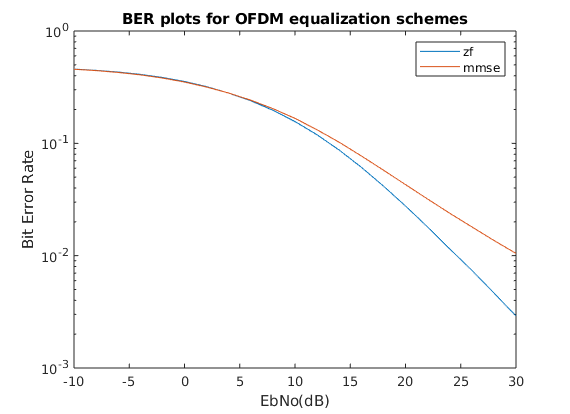
\includegraphics[scale=.4]{./media/ofdm_01.png}}
\caption{Comparing BER of different equalization schemes for OFDM over a Rayleigh fading channel}
\label{fig:ofdm}
\end{figure}\\ 
ZF proved to be a superior technique than mmse for higher SNR values. 
\section{Hybrid MIMO-OFDM System}
We combined the MIMO and OFDM systems into a single MIMO-OFDM wireless link. First, we construct an OFDM burst following the 802.11a standard. Then, we use an OFDM system with either ZF or MMSE equalization, and then decompose the signal into two and transmit through a 2x2 MIMO system and use either precoding, MMSE or ZF to reduce interference in the MIMO link. Note that the noise power for the awgn channel is evenly distributed between the two links. 
\subsection{Results}
We simulated a MIMO-OFDM system over three Rayleigh fading channels for our OFDM scheme and a flat-fading Gaussian channel for the MIMO system. We used a 16-QAM modulation scheme. For each equalization technique for OFDM channel equalization, we used each of the described MIMO methods for interference cancellation. Fig. \ref{fig:mimo-ofdm1} shows BER curves of the MIMO techniques for a ZF-OFDM scheme. Fig. \ref{fig:mimo-ofdm2} shows BER curves of the MIMO techniques for a MMSE-OFDM scheme.
\begin{figure}[htbp]
\centerline{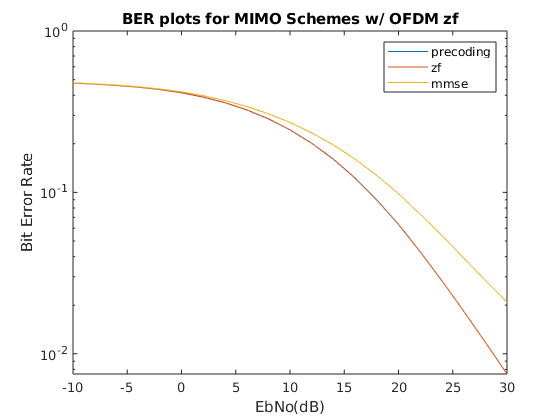
\includegraphics[scale=.4]{./media/mimo_ofdm_01.png}}
\caption{Comparing BER of different MIMO equalization schemes for a ZF-OFDM system}
\label{fig:mimo-ofdm1}
\end{figure}
\begin{figure}[htbp]
\centerline{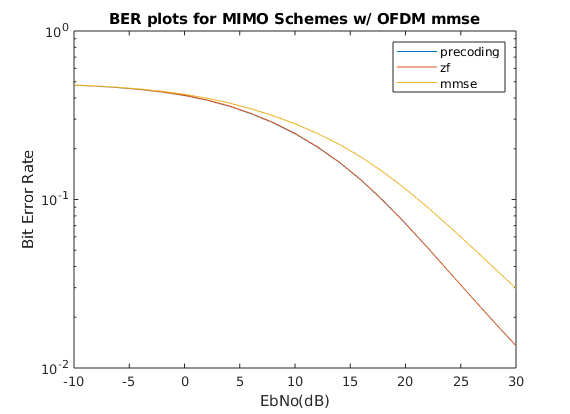
\includegraphics[scale=.4]{./media/mimo_ofdm_02.png}}
\caption{Comparing BER of different MIMO equalization schemes for a MMSE-OFDM system}
\label{fig:mimo-ofdm2}
\end{figure}\\ 
For both OFDM systems, precoding and ZF schemes for MIMO had nearly identical performance. ZF-OFDM proved superior to MMSE-OFDM in terms of bit error rate. Thus, the best wireless link is a ZF-MIMO with ZF-OFDM.
\section{Conclusion} 
We successfully simulated a MIMO wireless link and an OFDM scheme based on the IEEE802.11a PHY layer standard, experimenting with different methods for equalization and performance enhancement. We then implemented a hybrid MIMO-OFDM system and compared the performance of various equalization schemes.  

\bibliographystyle{unsrt}
\bibliography{bib}
\end{document}